\documentclass{article}
\usepackage{amsmath}
\usepackage{amssymb}
\usepackage{amsfonts}
\usepackage{pgfplots} 


\begin{document}
    \section*{1.3}
        \subsection*{a}
            $\Omega = \{1,\hdots,20\}^2$\\
            $\mathbb P: \Omega \rightarrow \mathbb R, (\omega_1, \omega_2) \mapsto \frac{1}{400}$
        \subsection*{b}
            \begin{enumerate}
                \item{$A = \{6\} \times \{1\hdots,20\}$\\
                    $\mathbb P (A) = \frac{1}{20}$}
                \item{$B = \{(6, 6)\}$\\
                    $\mathbb P (B) = \frac{1}{400}$}
                \item{$C = \{\{6\}\times \{1,\hdots 20\}, \{1,\hdots,5,7,\hdots,20\}\times\{6\}\}$\\
                    $\mathbb P(C) = \frac{39}{400}$}
                \item{$D = \{\{6\}\times \{1,\hdots 5,7,\hdots 20\}, \{1,\hdots,5,7,\hdots,20\}\times\{6\}\}$\\
                    $\mathbb P(C) = \frac{38}{400}$}
                \item{$E = \{\{1\}\times\{1,2,3\},\{2\}\times\{1,2\},\{3\}\times\{1\}\}$\\
                    $\mathbb P(E) = \frac{6}{400}$}
            \end{enumerate}

    \section*{1.4}
        \begin{tabular}{c|c}
            \textbf{$k$}&\textbf{$\mathbb P(X=k)$}\\
            \hline
            0&$\frac{1}{3}$\\
            1&$\frac{1}{2}$\\
            2&$0$\\
            3&$\frac{1}{6}$
        \end{tabular}\\
        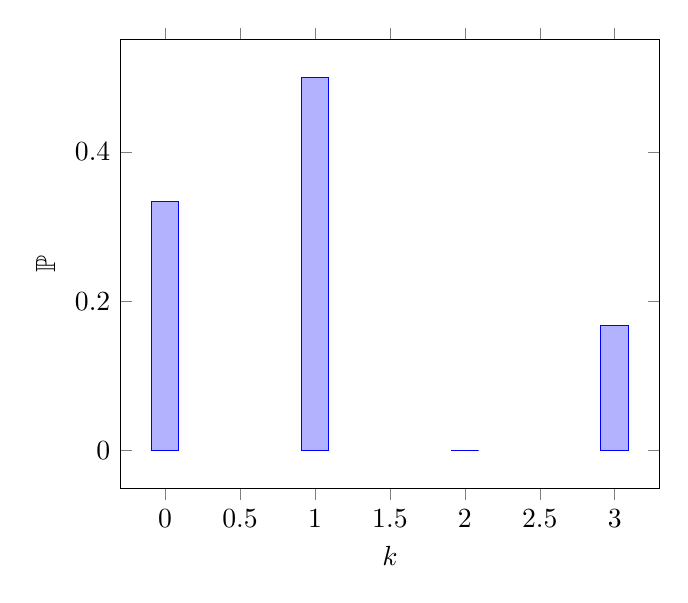
\begin{tikzpicture}
            \begin{axis} [ybar,xlabel=$k$,ylabel=$\mathbb P$]
                \addplot coordinates {
                    (0, 0.333) 
                    (1, 0.5) 
                    (2, 0) 
                    (3, 0.167)
                };
            \end{axis}
        \end{tikzpicture}
        \begin{tikzpicture}
            \begin{axis}[xlabel=k, ylabel=$F^X$]
                \addplot[color=blue] coordinates {
                    (-0.2,0) 
                    (0,0) 
                };
                \addplot[color=blue] coordinates {
                    (0, 0.333) 
                    (1,0.333) 
                };
                \addplot[color=blue] coordinates {
                    (1,0.833) 
                    (2,0.833) 
                };
                \addplot[color=blue] coordinates {
                    (2,0.833) 
                    (3,0.833) 
                };
                \addplot[color=blue] coordinates {
                    (3,1)
                    (3.2,1)
                };
                \addplot [only marks, mark size=2pt, color=blue]
                coordinates {
                        (0,0.333) 
                        (1,0.833) 
                        (2,0.833) 
                        (3,1)
                    };
            \end{axis}
        \end{tikzpicture}

    \newpage
    \section*{1.5}
        \begin{tabular}{c|c}
            \textbf{$\omega\in\Omega$}&\textbf{$X(\omega)$}\\
            \hline
            1&4\\
            2&1\\
            3&0\\
            4&1\\
            5&4\\
            6&9
        \end{tabular}
        \begin{tabular}{c|c|c}
            \textbf{$\omega\in X(\Omega)$}&\textbf{$X^{-1}(\omega)$}&\textbf{$\mathbb P(\omega)$}\\
            \hline
            0&\{3\}&$\frac{1}{6}$\\
            1&\{2,4\}&$\frac{2}{6}$\\
            4&\{1,5\}&$\frac{2}{6}$\\
            9&\{6\}&$\frac{1}{6}$
        \end{tabular}

        \subsection*{a}
        \begin{tikzpicture}
            \begin{axis}[xlabel=k, ylabel=$F^X$]
                \addplot[color=blue] coordinates {
                    (-0.2,0) 
                    (0,0) 
                };
                \addplot[color=blue] coordinates {
                    (0,0.167) 
                    (1,0.167) 
                };
                \addplot[color=blue] coordinates {
                    (1,0.5) 
                    (4,0.5) 
                };
                \addplot[color=blue] coordinates {
                    (4,0.833) 
                    (9,0.833) 
                };
                \addplot[color=blue] coordinates {
                    (9,1)
                    (9.2,1)
                };
                \addplot [only marks, mark size=2pt, color=blue]
                coordinates {
                        (0,0.167) 
                        (1,0.5) 
                        (4,0.833) 
                        (9,1)
                    };
            \end{axis}
        \end{tikzpicture}
        \subsection*{b}
        \begin{itemize}
            \item{$\mathbb E = 1\cdot\frac{1}{3}+4\cdot\frac{1}{3}+9\cdot\frac{1}{6}=\frac{19}{6}\approx 3.17$}
            \item{$\mathbb V = 
            (0-\frac{19}{6})^2\cdot\frac{1}{6}+(1-\frac{19}{6})^2\cdot\frac{1}{3}+
            (4-\frac{19}{6})^2\cdot\frac{1}{3}+(9-\frac{19}{6})^2\cdot\frac{1}{6}=\frac{329}{36}\approx 9.14$}
            \item{$\mathbb P(X\leq\mathbb E(X))=\mathbb P(X=0)+\mathbb P(X=1)=\frac{1}{6}+\frac{1}{3}=\frac{1}{2}$}
        \end{itemize}
    \section*{1.6}
        \subsection*{a}
            \begin{tabular}{c|c|c}
                \textbf{$m$}&\textbf{Kombinationen}&\textbf{$\mathbb P(M=m)$}\\
                \hline
                1&$\{1\}^{10}$&$(\frac{1}{6})^{10}\approx 1.66\cdot 10^{-8}$\\
                2&$\{(2)\times\{1,2\}^9, (1)\times(2)\times\{1,2\}^8,\hdots,\{1,2\}^9\times(2)\}$&$\frac{1}{6}\cdot(\frac{2}{6})^9\cdot 6\approx 5.08\cdot 10^{-5}$\\
                3&$\{(3)\times\{1,2,3\}^9, \{1,2\}\times(3)\times\{1,2,3\}^8,\hdots,\{1,2,3\}^9\times(3)\}$&$\frac{1}{6}\cdot(\frac{3}{6})^9\cdot 6\approx 0.002$\\
                4&$\vdots$&$\frac{1}{6}\cdot(\frac{4}{6})^9\cdot 6\approx 0.026$\\
                5&&$\frac{1}{6}\cdot(\frac{5}{6})^9\cdot 6\approx 0.194$\\
                3&&$1-\sum_{m\in 0\hdots 5}\mathbb P(M=m)\approx 0.778$
            \end{tabular}
            \begin{tikzpicture}
                \begin{axis}[xlabel=m, ylabel=$F^M$]
                    \addplot[color=blue] coordinates {
                        (0,0) 
                        (1,0)
                    };
                    \addplot[color=blue] coordinates {
                        (0,0.0) 
                        (1,0.0) 
                    };
                    \addplot[color=blue] coordinates {
                        (1,0) 
                        (2,0) 
                    };
                    \addplot[color=blue] coordinates {
                        (2,0) 
                        (3,0) 
                    };
                    \addplot[color=blue] coordinates {
                        (3,0.002) 
                        (4,0.002) 
                    };
                    \addplot[color=blue] coordinates {
                        (4,0.028) 
                        (5,0.028) 
                    };
                    \addplot[color=blue] coordinates {
                        (5,0.222) 
                        (6,0.222) 
                    };
                    \addplot[color=blue] coordinates {
                        (6,1) 
                        (6.2,1) 
                    };
                    \addplot [only marks, mark size=2pt, color=blue]
                    coordinates {
                            (0,0) 
                            (1,0) 
                            (2,0) 
                            (3,0.002) 
                            (4,0.028) 
                            (5,0.222) 
                            (6,1) 
                        };
                \end{axis}
            \end{tikzpicture}

    \section*{1.9}
        \subsection*{b}
            \begin{tabular}{c|c|c}
                \textbf{$Z$}&\textbf{Anzahl}&\textbf{W-keit}\\
                \hline
                -5&1&0.000231743\\
                -4&10&0.00386238\\
                -3&45&0.0269079\\
                -2&120&0.10128\\
                -1&210&0.222616\\
                0&252&0.290203\\
                1&210&0.222616\\
                2&120&0.10128\\
                3&45&0.0269079\\
                4&10&0.00386238\\
                5&1&0.000231743
            \end{tabular}

\end{document}